\section{Conceptualização}

De forma a atingir os objetivos propostos, foi necessário desenvolver um sistema
dividido em Motor Grafico e Gerador de Primitivas. O Motor Gráfico é responsável
por gerir e renderizar a cena e os modelos geométricos, enquanto que o Gerador de Primitivas
é responsável por criar as primitivas geométricas que compõem os modelos. 


\subsection{Modelo de Domínio}

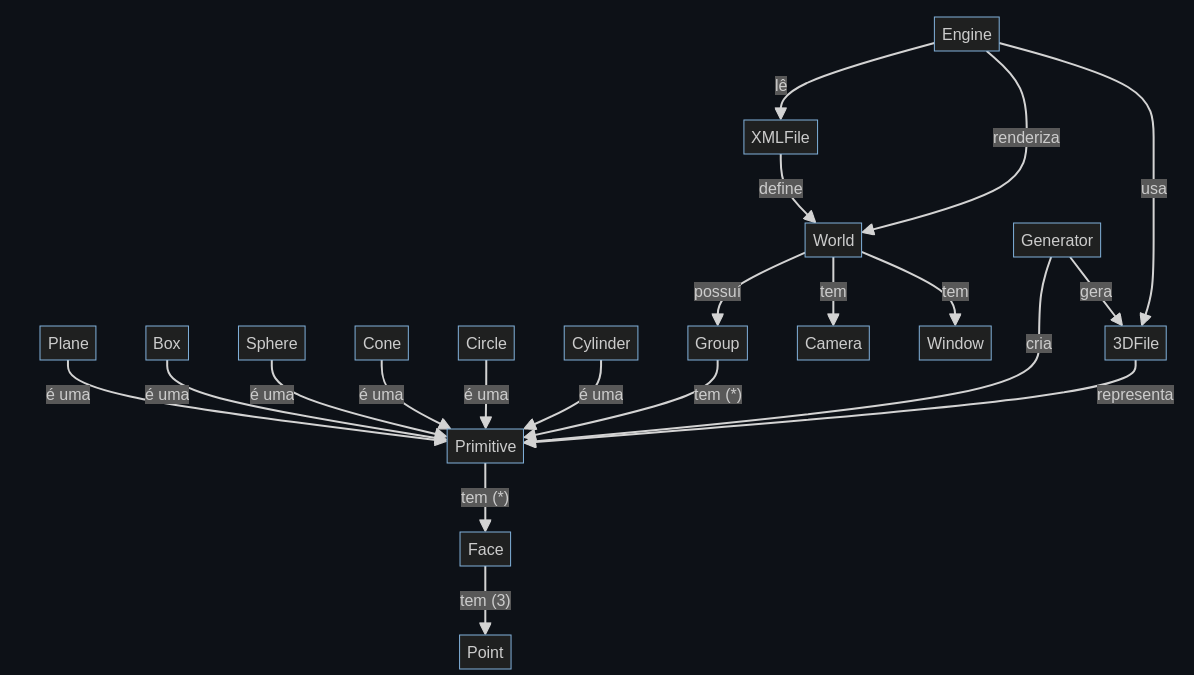
\includegraphics[width=15cm]{ModeloDominio.png}\\[\bigskipamount]

\subsection{Motor Gráfico}

Para atribuir uma organização ao sistema, foi decidido atribuir ao Motor Gráfico a
responsabilidade de ler ficheiros XML que descrevem a cena e os modelos ao que chamamos 
World. O World é composto por um grupo de primitivas, que por sua vez são
desenhados na prespetiva de uma câmara e uma janela.

\subsection{Gerador de Primitivas}

O Gerador de Primitivas é responsável por criar as primitivas geométricas que serão
transformadas em Ficheiros .3d e posteriormente lidos pelo Motor Gráfico para
quando este renderizar a cena.

